\chapter{L'oscillateur de Van der Pol}
%
On s'intéresse ensuite à l'équation de Van der Pol. Un modèle formulé par le physicien Balthasar van der Pol
pendant ses travaux sur des circuits électriques non-linéaires utilisées dans les premières radios \cite{strogatz_nonlinear_2015}.
%
\begin{equation}
    \ddot{x} + x + \epsilon(x^2 - 1)\dot{x} = 0
    \label{eq:vdp}
\end{equation}
%
C'est un système non conservatif avec une particularité intéressante. 
Le signe du terme d'amortissement $\epsilon(x^2 - 1)\dot{x}$ change en fonction de $x$. 
Lorsque $|x|<1$, le coefficient d'amortissement négatif fournit de l'énergie au système, et dans le cas contraire $|x|>1$, il en dissipe. 
Ce comportement particulier donne lieu a des oscillations entretenues de manière autonome.
On peut d'ailleurs retrouver ce terme non-linéaire dans l'équation de mouvement approximé d'un métronome, 
simulant l'effet du mécanisme d'horlogerie à échappement \cite{wang_-phase_2018}.

%
\begin{figure}[t]
    \centering
    \begin{subfigure}[b]{0.9\textwidth}
        %\hfill
        \begin{subfigure}[b]{.47\textwidth}
            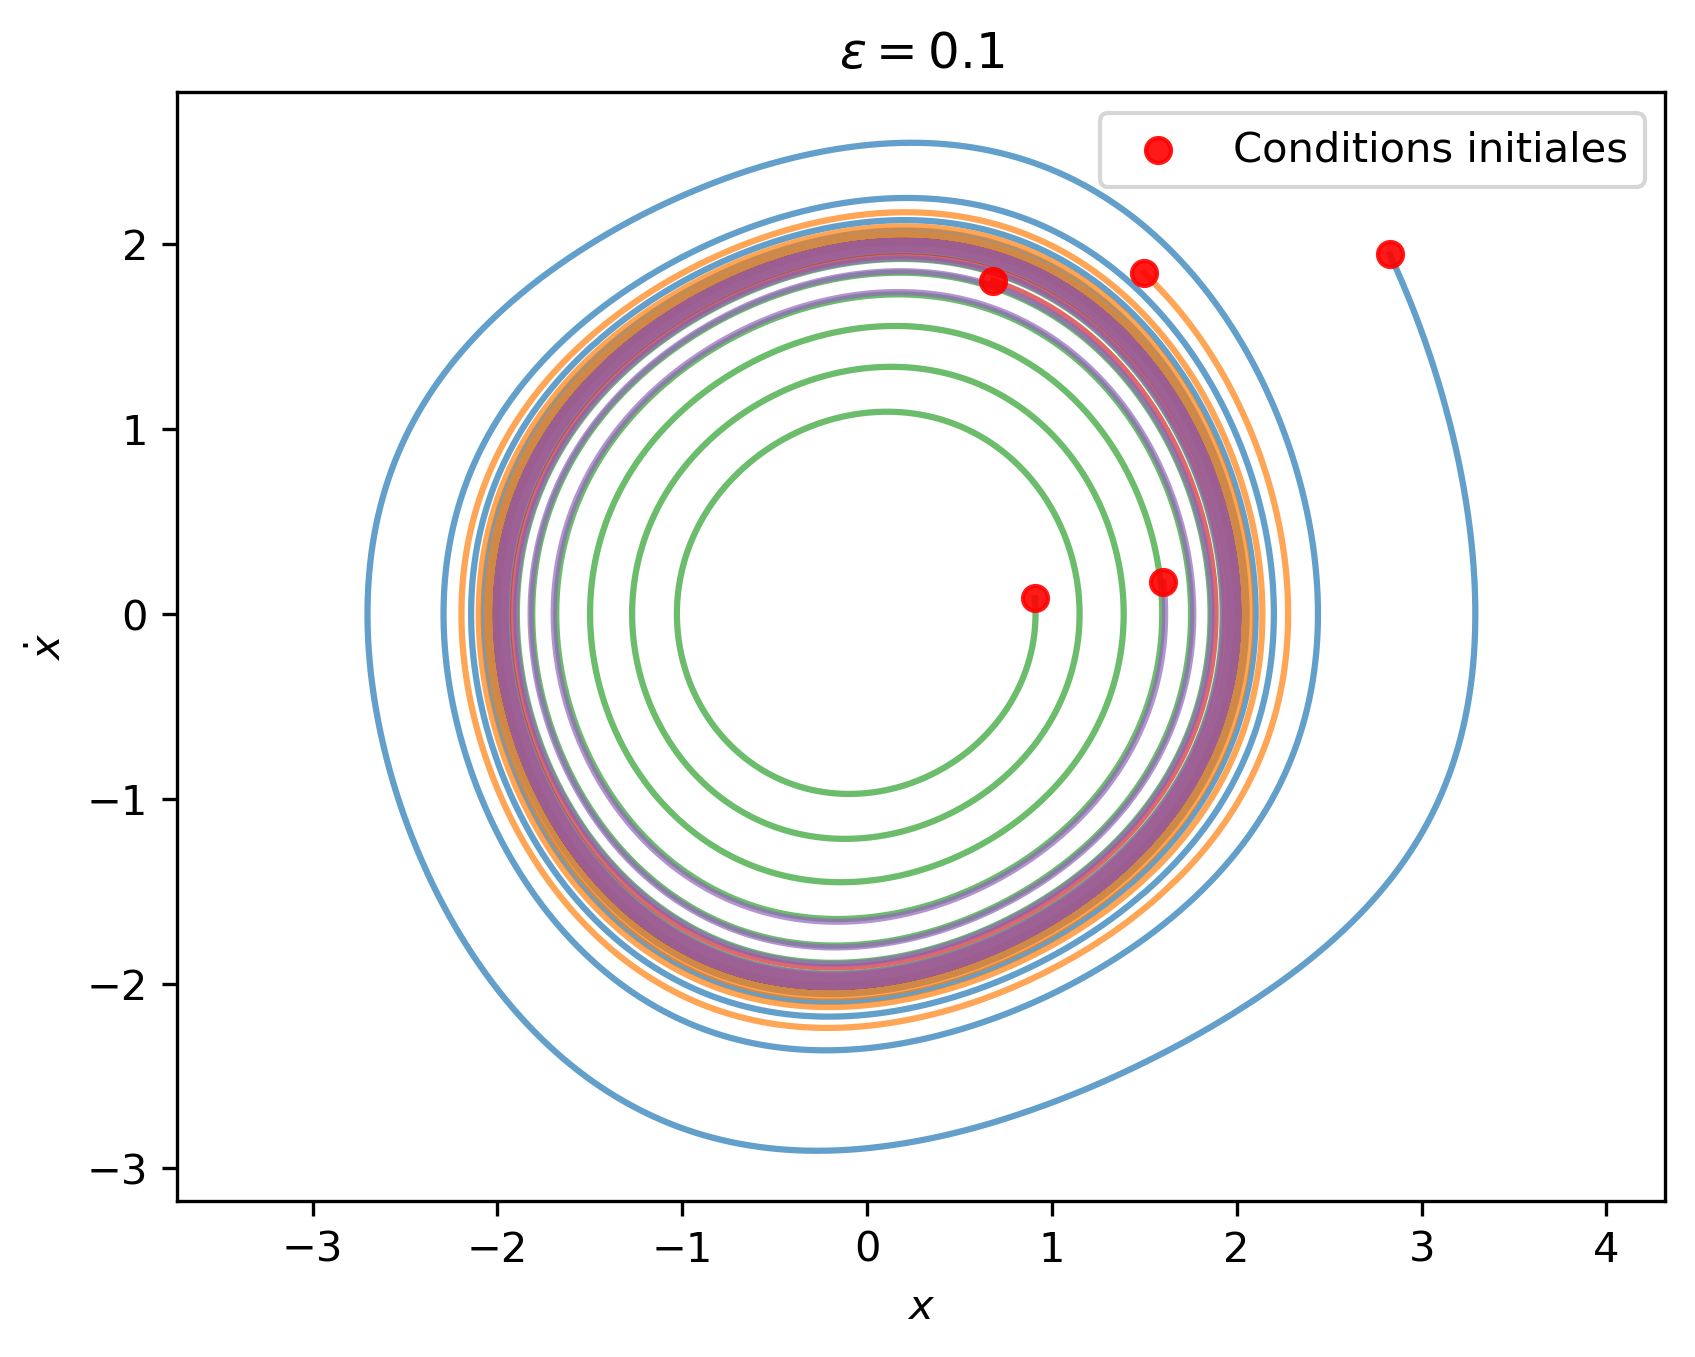
\includegraphics[width=\textwidth]{images/vdp/vanderpol_small.png}%
            \caption{}
        \end{subfigure}
        \hfill
        \begin{subfigure}[b]{.47\textwidth}
            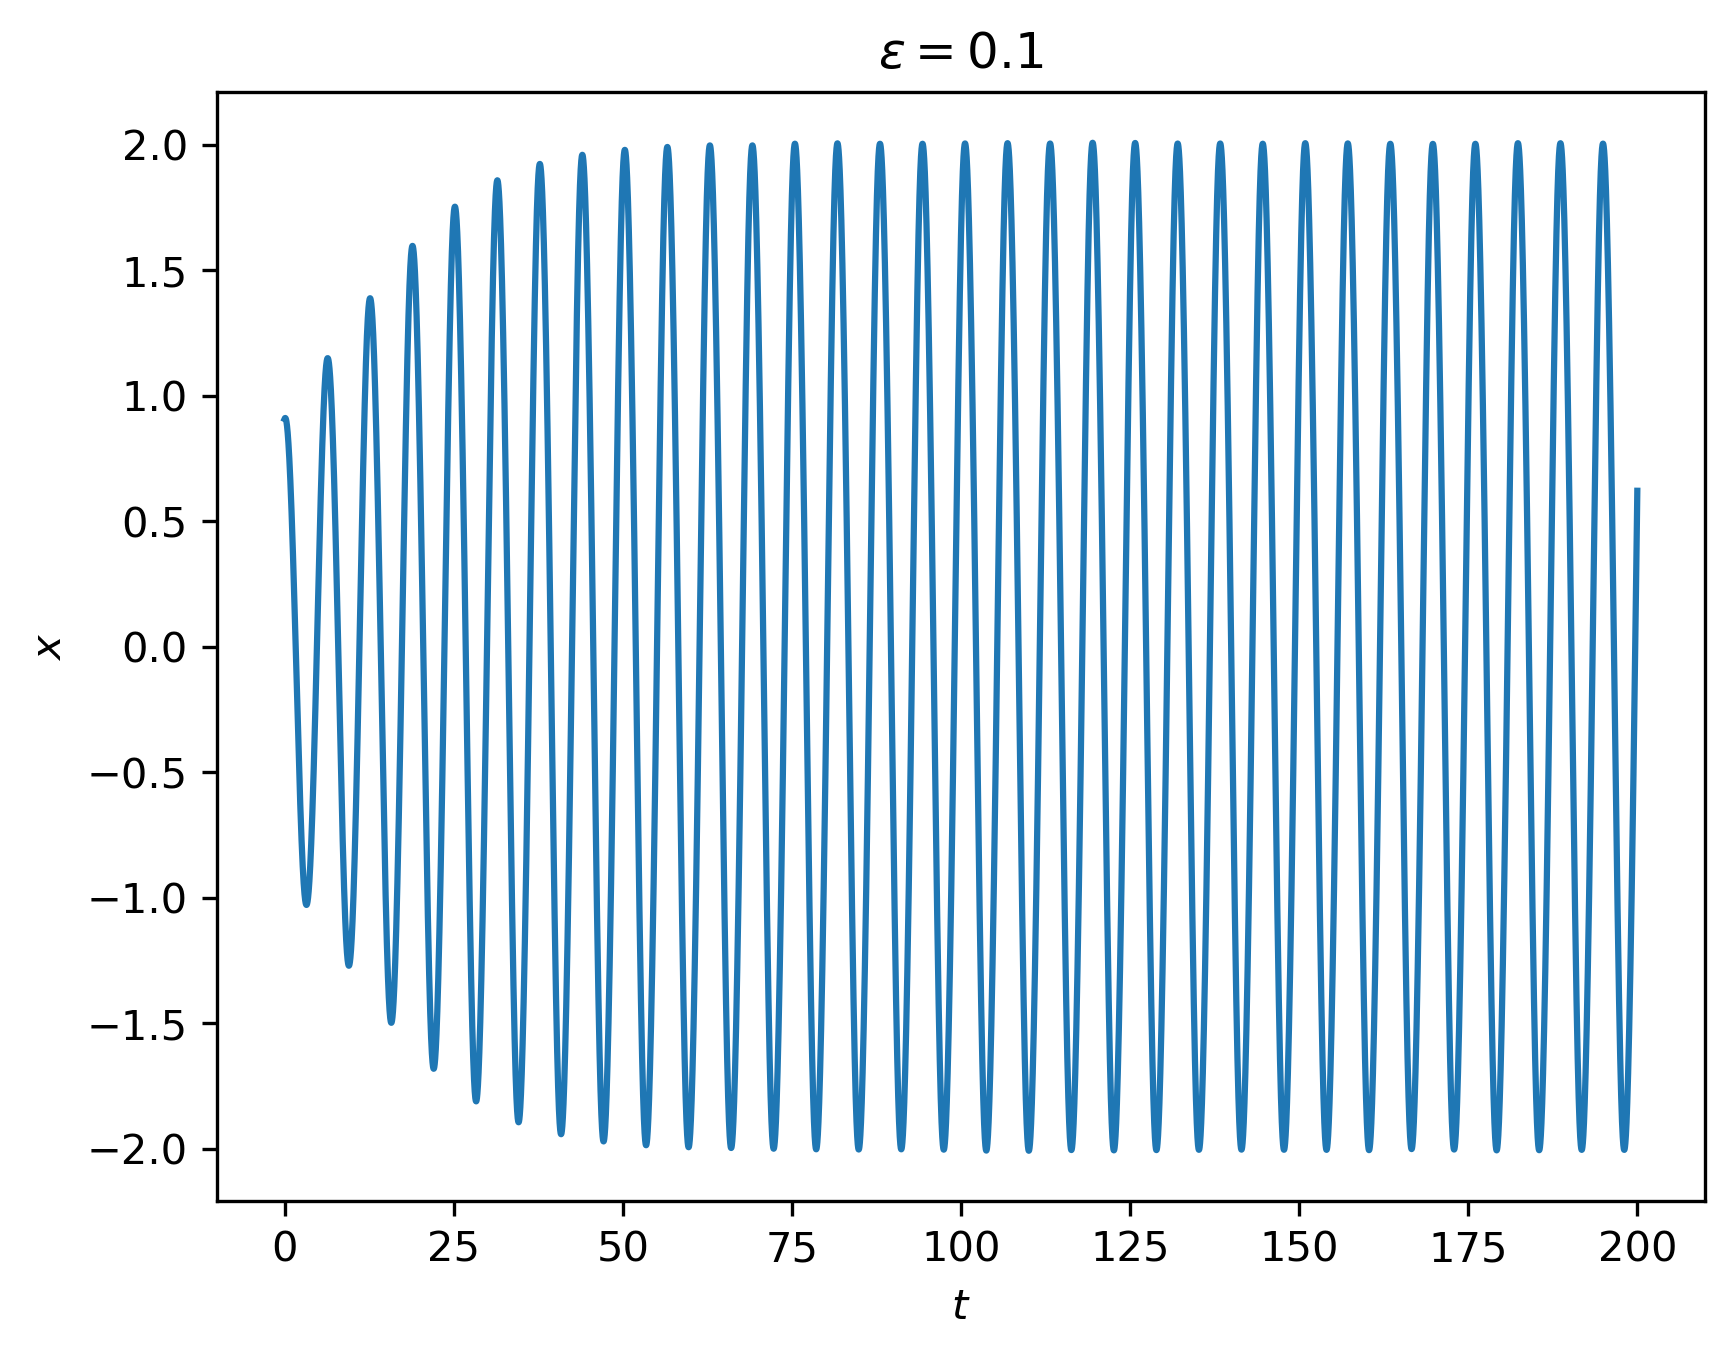
\includegraphics[width=\textwidth]{images/vdp/vanderpol_small_x.png}%
            \caption{}
        \end{subfigure}
        %\caption{}
    \end{subfigure}
    %\hfil
    \centering
    \begin{subfigure}[b]{0.9\textwidth}
        \begin{subfigure}[b]{.47\textwidth}
            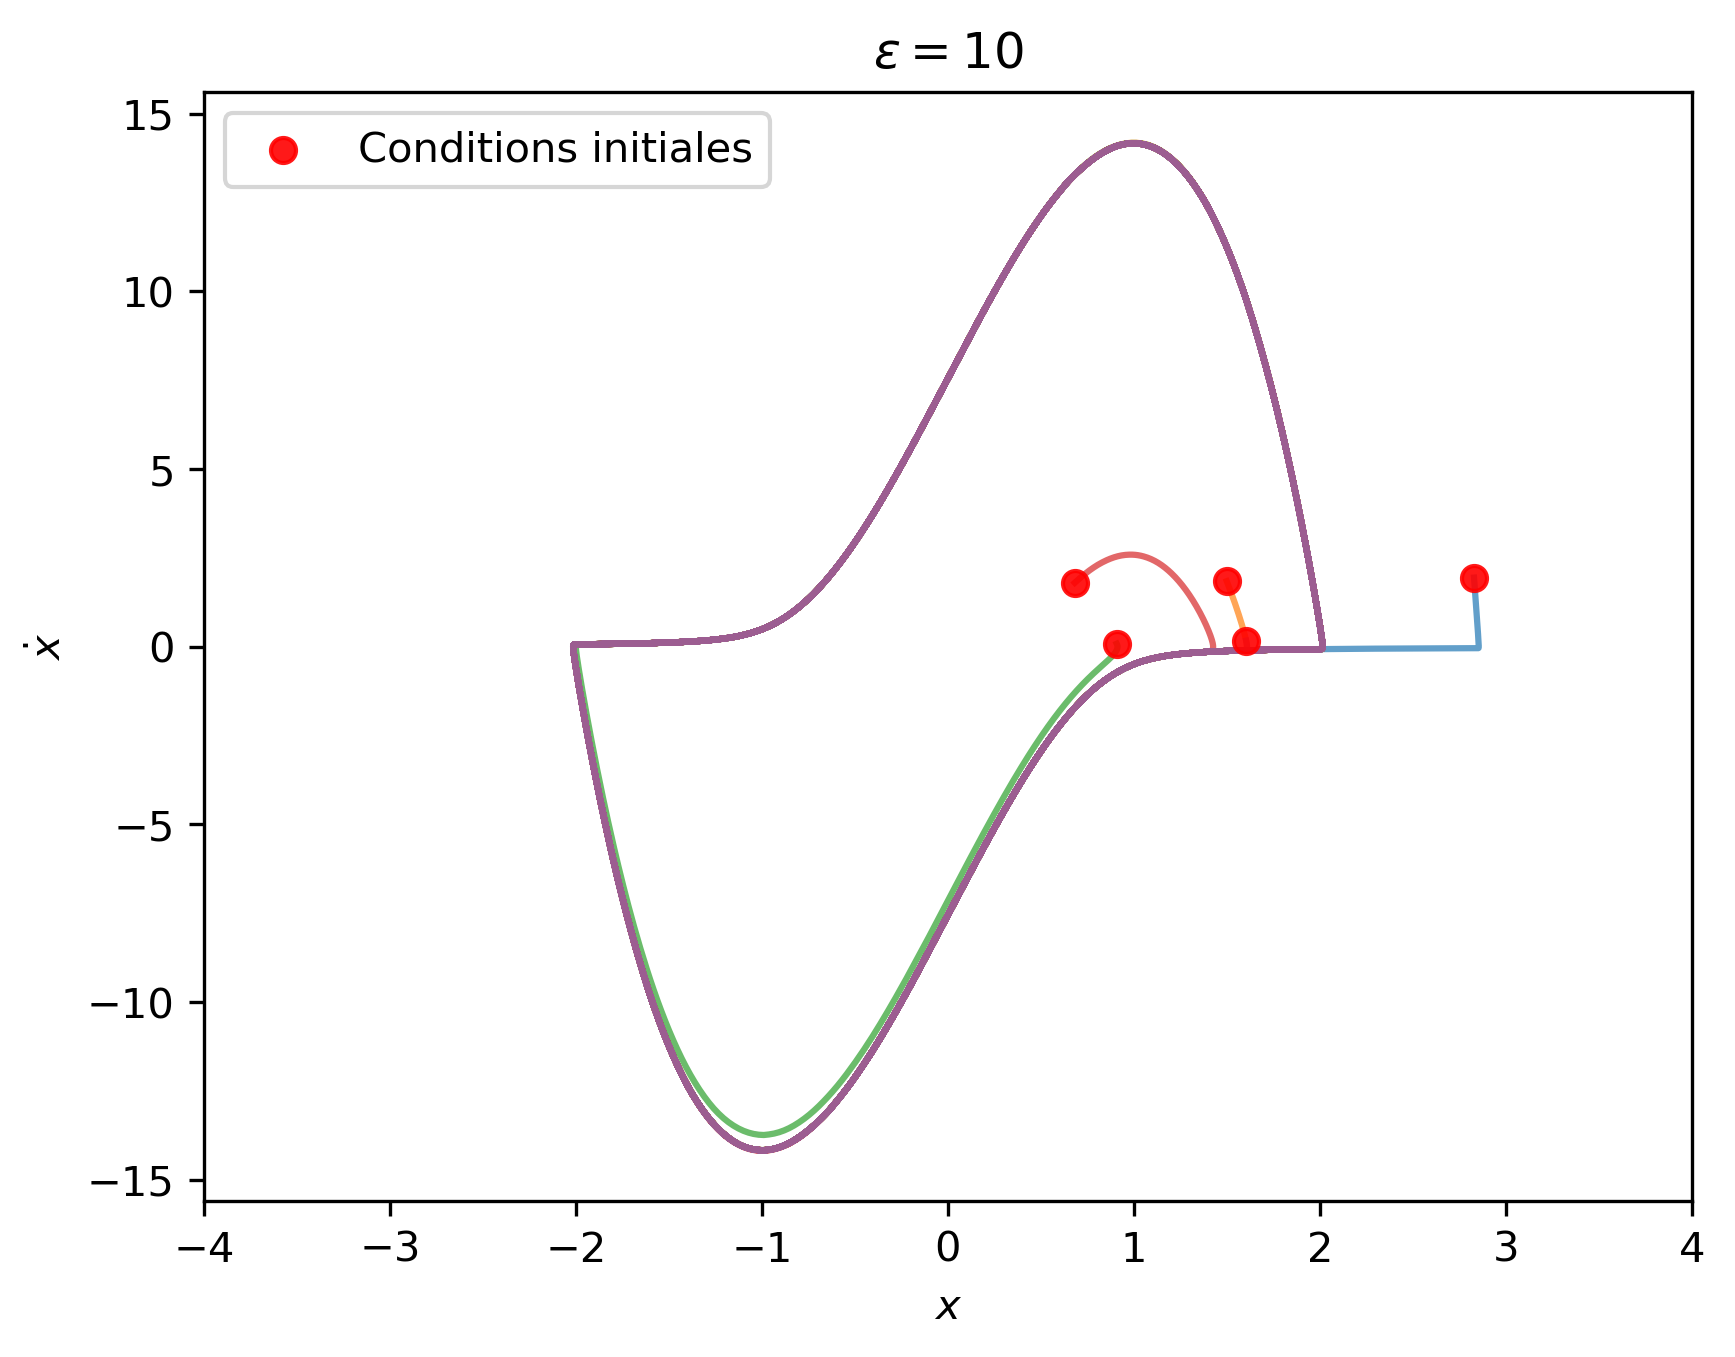
\includegraphics[width=\textwidth]{images/vdp/vanderpol_large.png}%
            \caption{}
        \end{subfigure}
        \hfill
        \begin{subfigure}[b]{.47\textwidth}
            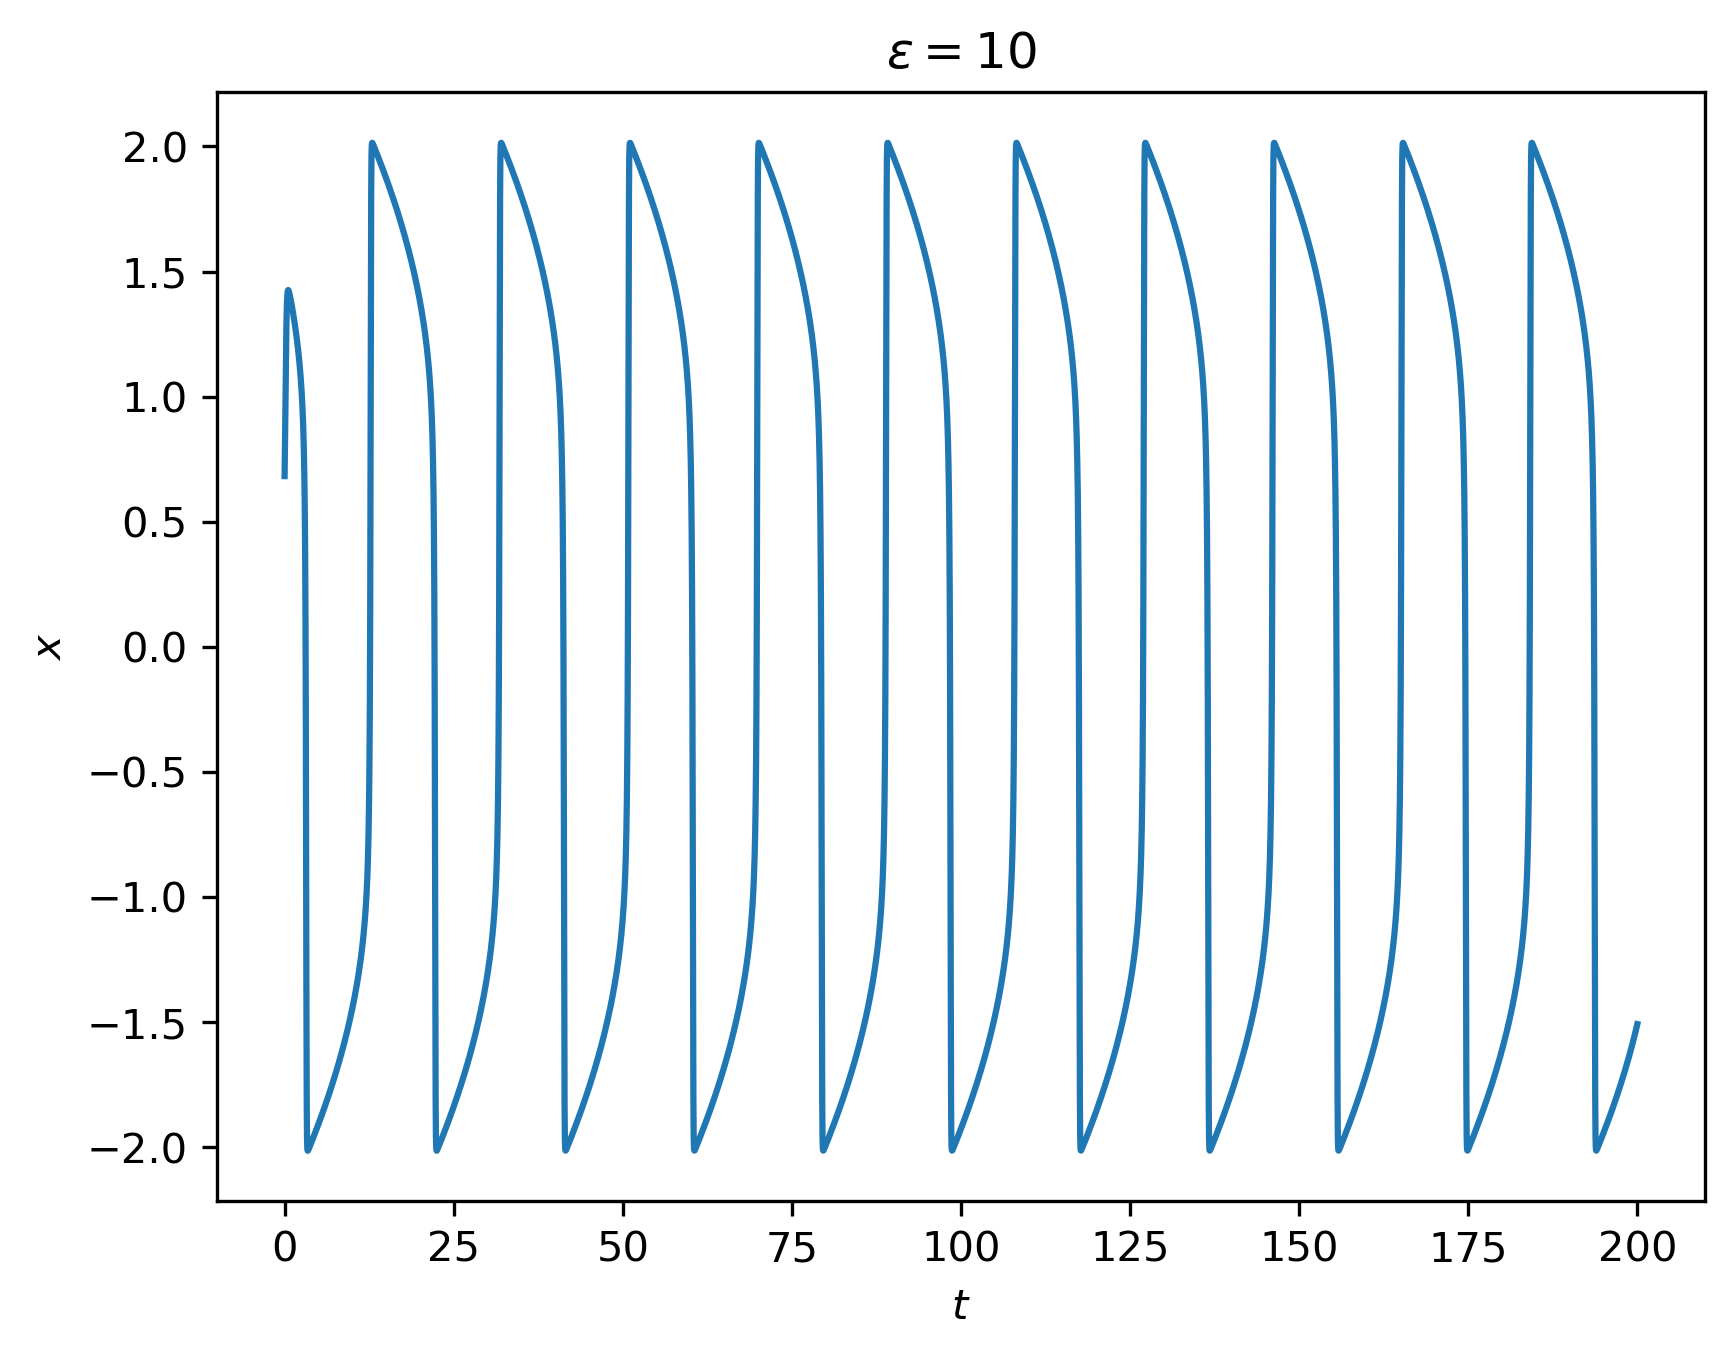
\includegraphics[width=\textwidth]{images/vdp/vanderpol_large_x.png}%
            \caption{}
        \end{subfigure}
        %\caption{$\epsilon = 5$}
        %\caption{}
    \end{subfigure}
    %
    \caption{Portraits de phase et tracés de l'amplitude de l'oscillateur de Van der Pol, obtenus par intégration numérique avec conditions initiales aléatoires \textbf{(a)} Portrait de phase, $\epsilon=0.1$ \textbf{(b)} Traçé $x$ contre $t$, $\epsilon=0.1$ \textbf{(c)} Portrait de phase, $\epsilon=10$ \textbf{(d)} Traçé $x$ contre $t$, $\epsilon=10$}\label{fig:portrait_vdp}
\end{figure}
%
%
Avec une étude numérique du système sur le plan de phase, on constate qu'il tend vers une unique orbite isolée, quelles que soient les conditions initiales imposées. 
Une telle orbite dans l'espace de phase s'appelle un \emph{cycle limite}. On voit notamment que pour petit $\epsilon$, le cycle limite est quasi-circulaire, 
alors que pour grand $\epsilon$ le cycle est fortement déformé et caractérisé par des oscillations de relaxations \cite{rand_lecture_2012}.
%c'est une oscillation de relaxation a cause des 
%De ce fait, il est possible de faire une analyse énergetique rudimentaire du système, en supposant que 
%
\section{Étude du cycle limite}
%
%Cette remarque, faite en premier par Lindstedt, va nous inspirer à chercher une solution approximative de \eqref{eq:vdp} sous forme d'un development perturbative
On cherche une solution approximative pour le cycle limite de \eqref{eq:vdp} sous forme d'un développement perturbative valide pour $\epsilon \ll 1$. 
En comparant les systèmes faiblement et fortement non-linéaire (fig. \ref{fig:portrait_vdp}), on observe que la fréquence d'oscillation diverge de la fréquence naturelle $\omega_0 = 1$ lorsque $\epsilon$ augmente. 
En raison de cela, on va utiliser la méthode de Lindstedt \cite{rand_lecture_2012}, 
qui nous permet de prendre en compte la dépendance de la fréquence d'oscillations sur $\epsilon$. 

L'approche consiste à définir une échelle de temps dilaté $\tau$ et de prendre la fréquence $\omega$ du cycle limite comme étant un inconnu qui dépend de $\epsilon$ :
\begin{equation}
    \tau = \omega t
    \qquad
    \omega(\epsilon) = \omega_0 + \epsilon\omega_1 + \epsilon^2\omega_2 + O(\epsilon^3)
    \label{eq:omega_eps}
\end{equation}
%
En résolvant l'équation sous cette nouvelle échelle de temps, on permet à la solution approximative de prendre compte de ce décalage de fréquence.
Ce que la méthode perturbative classique ne peut pas faire.
%La justification derrière cette transformation d'echelle est qu'elle donne à notre solution approximative la possibilité d'avoir une fréquence dépendante de $\epsilon$.
%La justification derrière cette transformation d'echelle de temps est qu'elle nous permet de définir $x(\tau)$ comme étant $2\pi$ periodique, 
%alors que $x(t)$ à une periode qui nous est encore inconnue en raison de sa dépendence sur $\omega$.
\begin{equation}
    x(\tau, \epsilon) = x_0(\tau) + \epsilon x_1(\tau) + \epsilon^2 x_2(\tau) + O(\epsilon^3)
    \label{eq:x_eps}
\end{equation}
%
Les termes à l’ordre zéro dans les développements correspondent aux solutions de \eqref{eq:vdp} lorsque $\epsilon = 0$.
Ce sont les termes de base que l’on va chercher à ``perturber” avec des petits termes correcteurs.
%
Suite à la transformation d'échelle $x(t) \to x(\tau)$, \eqref{eq:vdp} devient :
%
\begin{equation}
    \omega^2x''(\tau) + x''(\tau) + \epsilon\omega \left( x(\tau)^2 - 1 \right)x'(\tau) = 0
    \label{eq:vdp_linsted}
\end{equation}
%
Où le prime dénote une dérivée par rapport à $\tau$. En substituant \eqref{eq:omega_eps} et \eqref{eq:x_eps} dans \eqref{eq:vdp_linsted} :
%
\begin{dmath}
    (1+\epsilon\omega_1 + \epsilon^2\omega_2)^2(x_0'' + \epsilon x_1'' + \epsilon x_2'') + \epsilon(1+\epsilon\omega_1 + \epsilon^2\omega_2)\left[(x_0 + \epsilon x_1 + \epsilon^2 x_2)^2-1\right](x_0' + \epsilon x_1' + \epsilon^2 x_2') \\
    + {x_0 + \epsilon x_1 + \epsilon^2 x_2} = 0
\end{dmath}
%
On s’attend à ce que cette  équation soit valide pour tout $\epsilon$, donc les coefficients de $\epsilon^n$ doivent s’annuler indépendamment les un des autres. 
En négligeant les termes $O(\epsilon^3)$ et en regroupant les coefficients de $\epsilon^n$ on obtient les trois équations suivantes :
%
\begin{align}
    \label{eq:O_1}
    O(\epsilon^0)\text{:}\qquad      x_0'' + x_0 &= 0  \\
    \label{eq:O_eps}
    O(\epsilon^1)\text{:}\qquad      x_1'' + x_1 &= -2\omega_1 x_0'' - (x_0^2 - 1)x_0' \\
    \label{eq:O_eps2}
    O(\epsilon^2)\text{:}\qquad      x_2'' + x_2 &= -2\omega_2 x_1'' - (2\omega_2 + \omega_1^2)x_0'' - (x_0^2 - 1)x_1' - 2x_0 x_1 x_0' - \omega_1(x_0^2 - 1)x_0'
\end{align}
%
%A cause de la periodicité de notre solution, on peut, sans perdre de géneralité, imposer les conditions initiales suivantes.
%
On peut constater que si on impose des conditions initiales arbitraires $x(0, \epsilon)=A,  \, x'(0, \epsilon)=B$, pour que \eqref{eq:x_eps} 
soit valide pour tout $\epsilon$ il faut obligatoirement que :
%
\begin{equation}
    x_0(0) = A,\, x_0'(0) = B
    \qquad
    x_k(0) = x_k'(0) = 0 \; \forall k > 0
\end{equation}
%
On commence donc par résoudre \eqref{eq:O_1}, qui correspond à l'oscillateur harmonique de base :
%
\begin{equation}
    x_0(\tau) = A \cos(\tau + \phi_B)
\end{equation}
%
En raison de la nature autonome de \eqref{eq:O_1} (l'absence explicite du temps), on est libre de choisir l'origine du temps de telle sorte à éliminer la phase $\phi_B$, 
ce qui est équivalent à imposer la condition $B = 0$. On résout alors \eqref{eq:O_eps} en y substituant l’expression de $x_0$ :
%
\begin{dmath}
    x_1'' + x_1 = 2\omega_1 A \cos(\tau) + (A^2 \cos^2(\tau) - 1)A\sin(\tau) \\
    = 2\omega_1 A \cos(\tau) + (\frac{1}{4}A^3 - A)\sin(\tau) + \frac{1}{4}A^3 \sin(3\tau)
\end{dmath}
%
On remarque la présence de termes résonants (aussi appelés termes séculaires) de type $k\cos(\tau)$ et $k\sin(\tau)$ dans l'équation. 
Or, si on cherche à trouver une solution periodique, les coefficients de ces termes résonants doivent s'annuler.
En effet, ils donnent lieu à des solutions de la forme $k' \tau \sin(\tau)$ qui ne sont pas bornées avec le temps.
En appliquant cette condition de périodicité :
%
\begin{equation}
    2\omega_1 A  = 0
    \qquad
    \frac{1}{4}A^3 - A = 0
\end{equation}
%
$A=0$ correspond à la solution stationnaire instable du système et $A=-2$ correspond à une différence de phase de $\pi$ par rapport à $A=2$. On conclut donc (sans perte de généralité) que $\omega_1 = 0$ et que $A=2$. 
Selon la dernière condition, on conclut que pour $\epsilon$ quelconque non-nulle, seule l'orbite circulaire de rayon $2$ (sur le plan de phase) reste solution periodique.
%La dernière condition en particulier nous dit que dès que $\epsilon$ devient non-nulle, seule l'orbite circulaire de rayon $2$ (sur le plan de phase) reste possible.
%toutes les orbites circulaires sur le plan de phase sont détruits, sauf celui avec un rayon de $2$. 
En effet, le système converge vers une unique solution periodique - un cycle limite.

Ensuite, on résout $x_1'' + x_1 = 2\sin(3\tau)$ en appliquant les conditions initiales :
\begin{equation}
    x_1 = \frac{3}{4}\sin(\tau) - \frac{1}{4}\sin(3\tau)
\end{equation}
%
Et on répète le processus en substituant les expressions de $\omega_1$, $A$ et de $x_1$ dans \eqref{eq:O_eps2} :
%
\begin{dmath}
    x_2'' + x_2 = 4\omega_2\cos(\tau) + 8\sin(\tau)\cos(\tau)\left(\frac{3}{4}\sin(\tau) - \frac{1}{4}\sin(3\tau)\right) - \left(\frac{3}{4}\cos(\tau) - \frac{3}{4}\cos(3\tau)\right)(4\cos^2(\tau)-1) \\
    = (4\omega_2 + \frac{1}{4})\cos(\tau) - \frac{3}{2}\cos(3\tau) + \frac{5}{4}\cos(5\tau)
\end{dmath}
%
Donc, pour éliminer le terme résonant, il faut que $\omega_2 = -\frac{1}{16}$. On résout l'équation qui en résulte pour trouver :
%
\begin{equation}
    x_2(\tau) = \frac{3}{16}\cos(3\tau) - \frac{5}{96}\cos(5\tau) - \frac{41}{304}\cos(\tau)
\end{equation}
%
\begin{equation}
    \omega = 1 - \frac{1}{16}\epsilon^2 + O(\epsilon^3)
\end{equation}
%
\section{Étude de l'état transitoire}
%
\begin{comment}
    We now know the oscillation frequency for the limit cycle. 
    However we don't know how the oscillation frequency evolves as it reaches steady state.
    I suppose we just assume that the frequency of the oscillator during the transient period is just close enough
    to the steady state frequncy.
\end{comment}
%
On cherche maintenant à étudier
l'approche du système vers le cycle limite. Pour faire cela, on applique la méthode de moyennement. Pour $\epsilon \ll 1$, on prend
la fréquence d'oscillation $\omega = 1$ constante et on cherche de solutions sous la forme :
\begin{equation}
    x(t) = z(t)e^{it} + \bar{z}(t)e^{-it}
    \qquad
    \dot{x}(t) = i\left[ z(t)r^{it} - \bar{z}(t)e^{-it} \right]
    \label{eq:vdp_x_xdot}
\end{equation}
%
Avec :
%
\begin{equation}
    z(t) = \frac{r(t)}{2}e^{i\phi(t)}
\end{equation}
%
On substitue \eqref{eq:vdp_x_xdot} dans \eqref{eq:vdp} puis on applique le même raisonnement
que pour l'oscillateur de Duffing pour obtenir :
%
\begin{equation}
    2\dot{z}(t) =
    - \epsilon \left( z^2(t)\bar{z}(t) - z(t) \right)
\end{equation}
%
Sachant que $\dot{z}(t) = \frac{\dot{r}}{2}e^{i\phi} + i\dot{\phi}\frac{r}{2}e^{i\phi}$, on peut séparer la partie réelle et la partie imaginaire de l'équation pour obtenir le système :
\begin{equation}
    \left\{
    \begin{array}{@{}l@{}}
        \dot{r} = \frac{\epsilon}{8}r(4-r^2) \\
        \\
        \dot{\phi} = 0
    \end{array}
    \right.\,
\end{equation}
%
On fait l'observation que le système Van der Pol n'a pas de fréquence de référence - contrairement à l'oscillateur de Duffing forcé, la phase à l'état stable dépend que des conditions initiales.
On retrouve aussi les deux solutions stationnaires stable et instable à $r=2$ et $r=0$ trouvé auparavant avec la méthode de Linstedt. On peut résoudre la première équation par séparation des variables pour le cas $r \neq 2$ :
%
\begin{equation}
    r(t) = 2 \sqrt{ \frac{A}{A + e^{-\epsilon t}} }
    \qquad
    \text{Où}
    \qquad 
    A = \frac{r(0)^2}{4 - r(0)^2}
\end{equation}
%
\begin{figure}
    \centering
    \begin{subcaptionblock}{.90\linewidth}
        %\hfill
        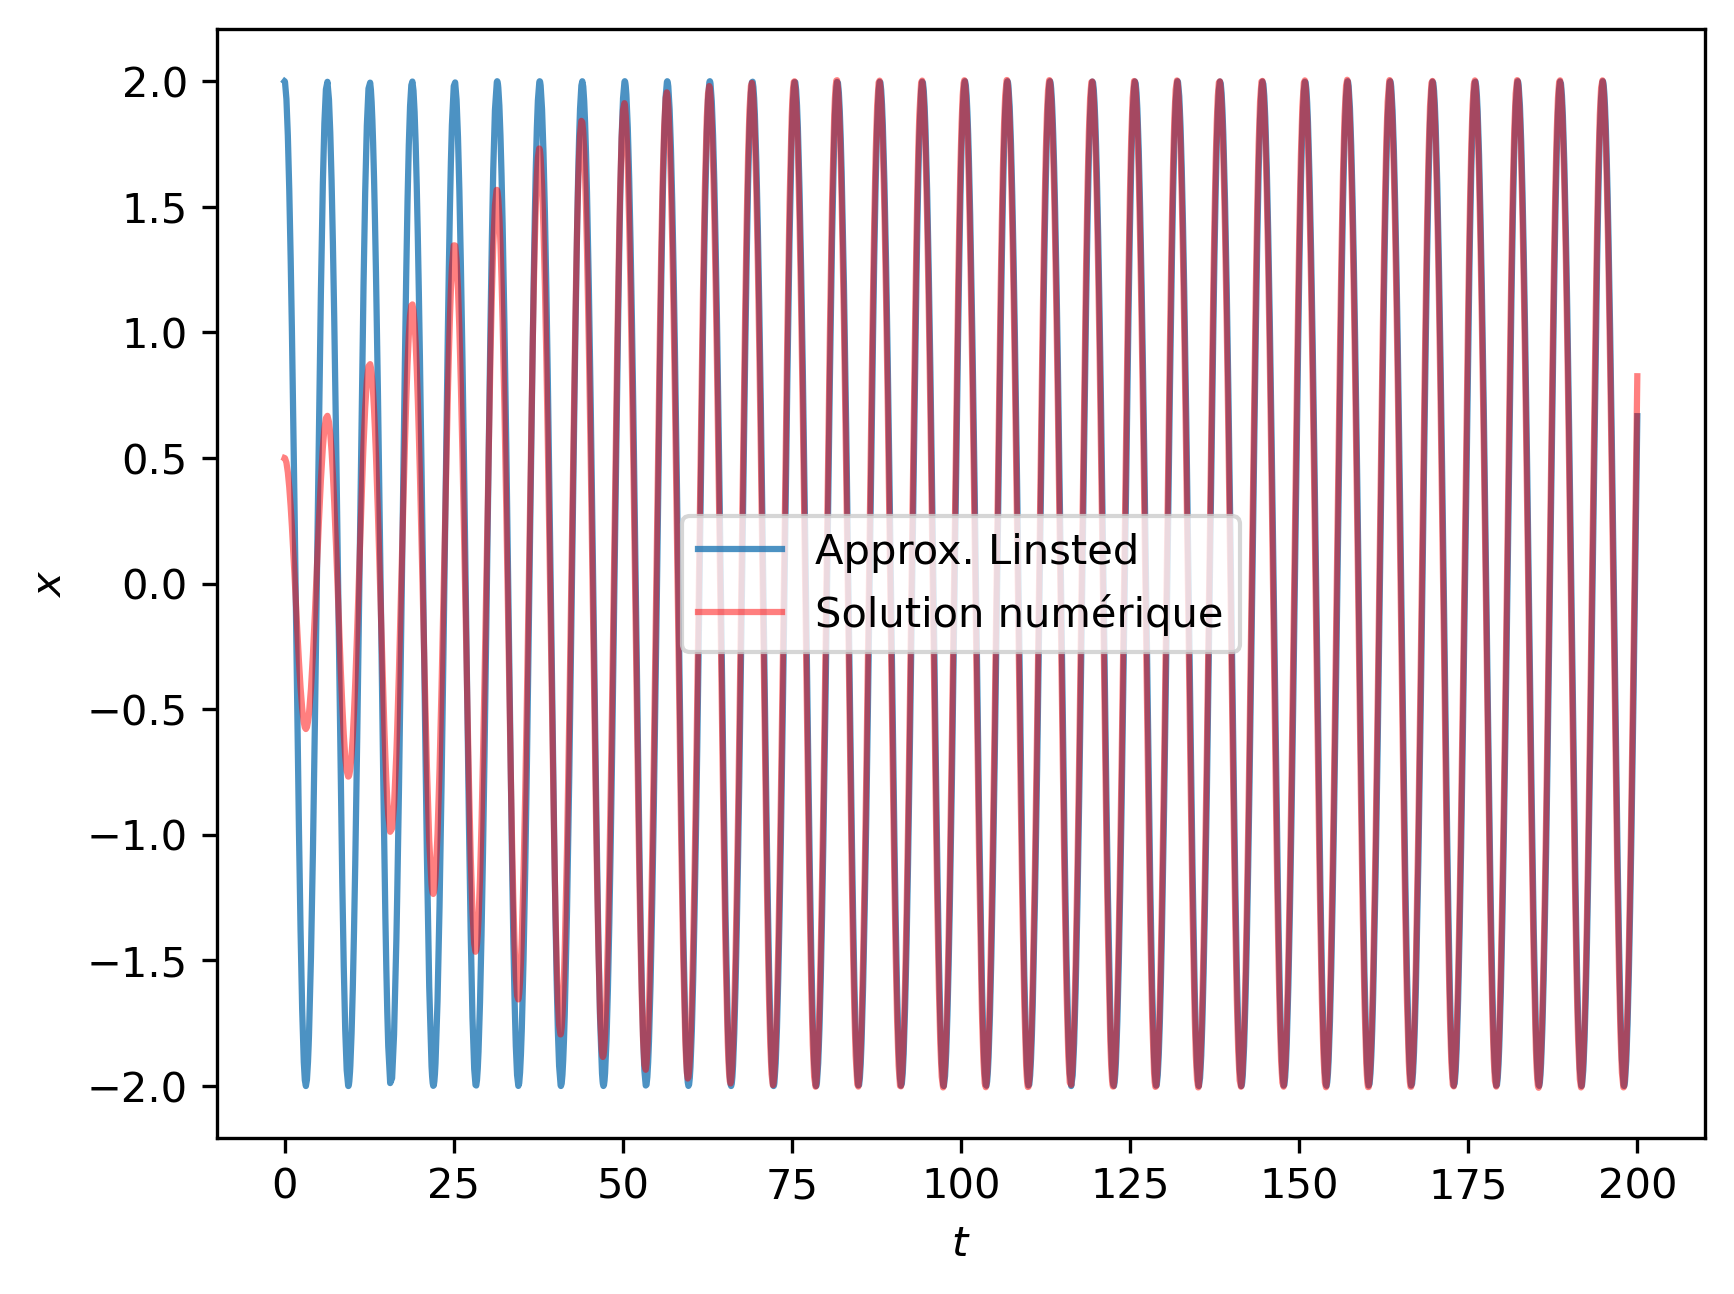
\includegraphics[width=.5\linewidth]{images/vdp/vdp_approx_linsted.png}%
        \hfill
        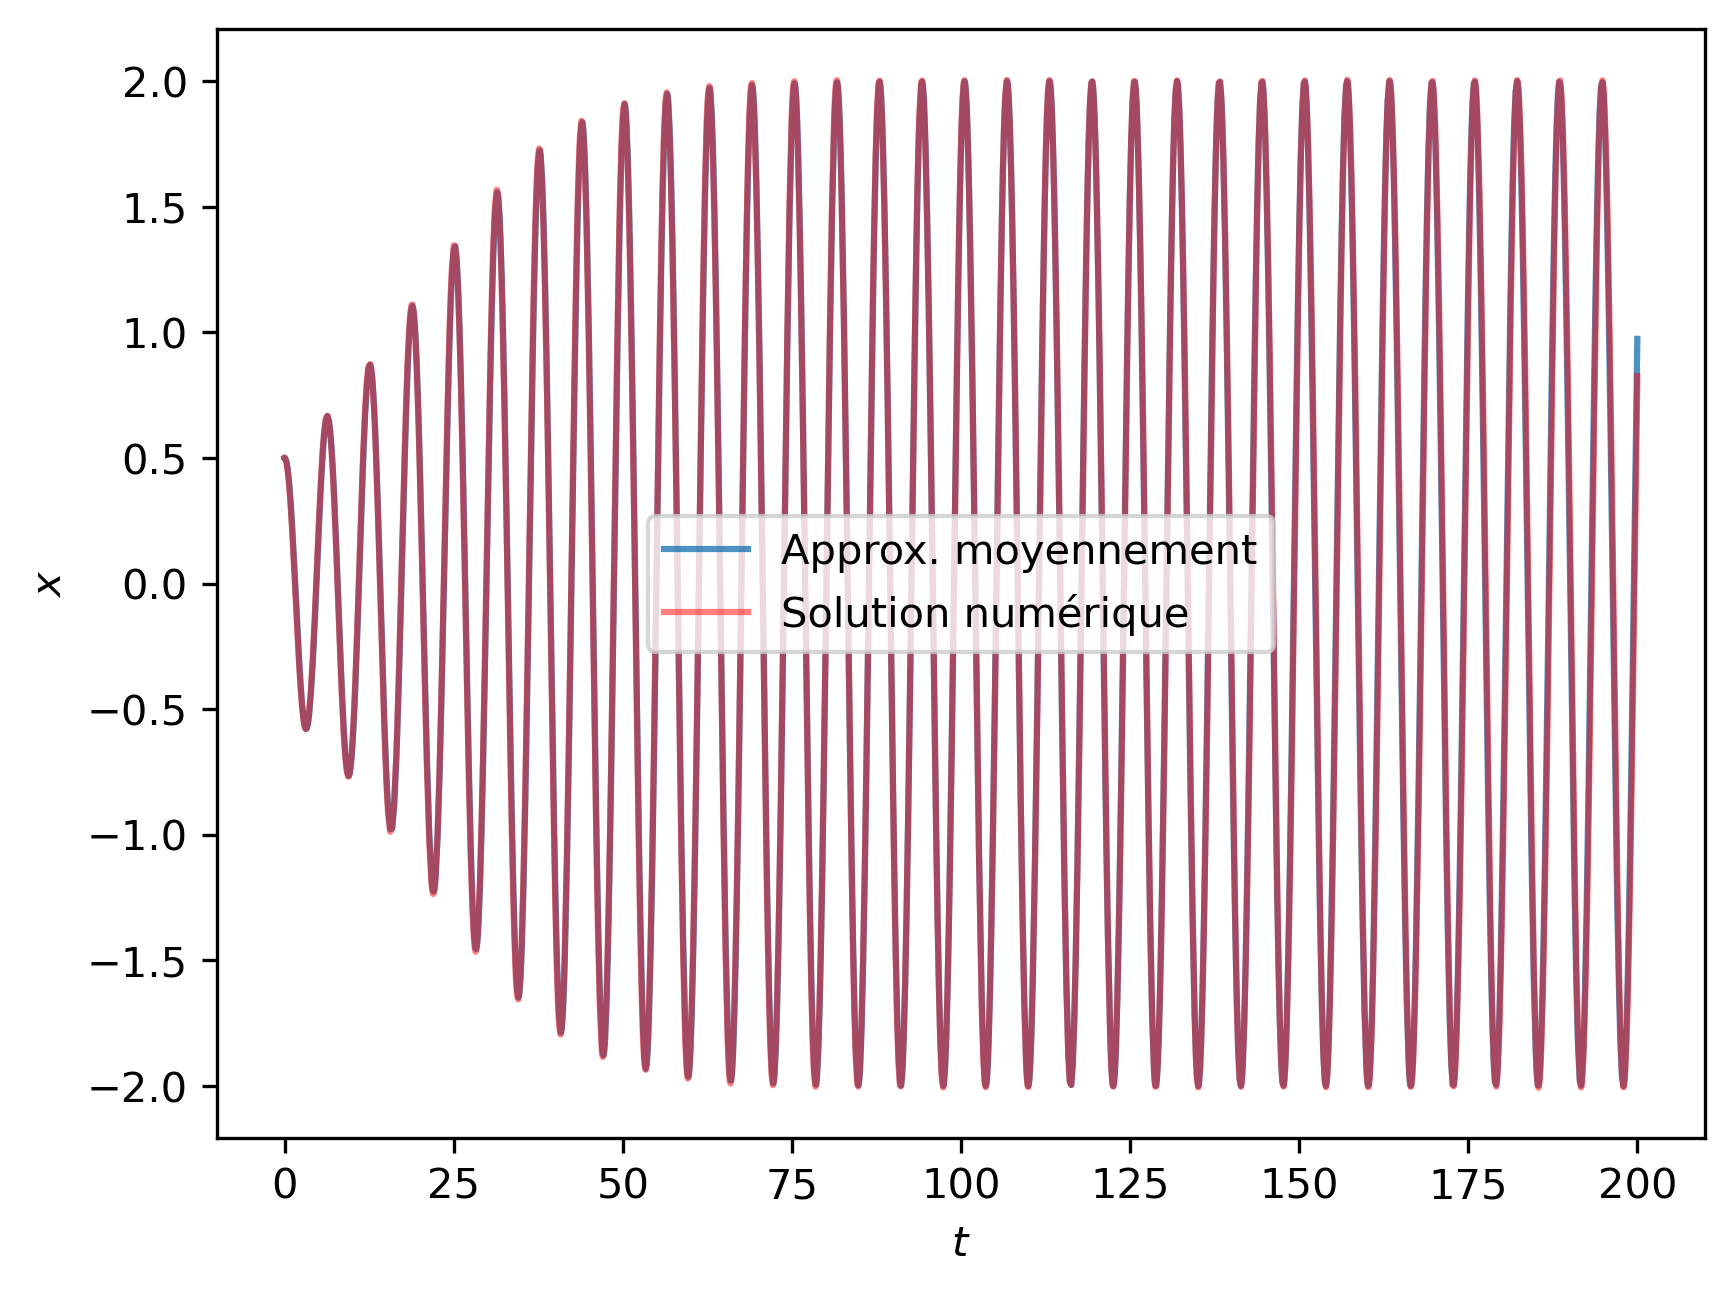
\includegraphics[width=.5\linewidth]{images/vdp/vdp_approx_transient.png}%
        %\hfill
        %\centering
        %\caption{$\epsilon = 0.1$}
    \end{subcaptionblock}
    \caption{Comparaison des deux approximations avec une solution numérique, $\epsilon=0.1$, $x(0)=0.5$, $\dot{x}(0)=0$}
    \label{fig:vdp_approx}
\end{figure}
%
Dans {fig. \ref{fig:vdp_approx}} on voit que l'approximation obtenue par le moyennement est légèrement en avance par rapport à la solution numérique, on peut attribuer cela à l'approximation $\omega \approx 1$ qui a été fait en négligeant les termes en $\epsilon^2$. 
De ce fait, l'approximation n'est que fiable jusqu'à des temps de l'ordre $O\left( \frac{1}{\epsilon^2} \right)$ car au-delà de ça le décalage entre la solution et l'approximation devient non négligeable.